% !Mode:: "TeX:UTF-8" 
\section{课题来源及研究的背景和意义}
\subsection{课题的来源}
服务计算的哲理之一是利用互联网上的海量候选服务进行组合,形成满足客户需求的大粒度服务。由于互联网环境的动态变化和不稳定特性,构建在其基础上的服务系统在执行过程中也面临各种不确定性,某些服务环节可能无法按照预期执行,供需双方期望的价值无法完全实现,还可能触发其他更多的不确定性事件,造成各种直接和潜在的影响。

本文将该“不确定性”定义为“某个已经或即将发生的事件,它使得服务实际执行结果与预先达成的服务级别协议~(Service Level Agreement, SLA)~之间产生了偏差”。服务执行中典型的不确定性事件包括:1) 某个服务环节执行之后未达到期望的质量~(QoS)~;2) 某个服务环节执行失败;3) 客户需求发生变更或完全取消;4) 可用服务/资源的数量或价格发生波动;5) 外部商业环境或政策发生变化,导致预设的服务流程失效;等等。从发生时间看,不确定性事件分为两种类型:已经发生并已造成影响的事件、预测将要发生但尚未发生的事件。

为了应对不确定性,核心策略就是“按需应变”:根据预期发生的或已经发生的不确定性,对服务做出调整。这里的“变”即各种不确定性事件,“应”即所采取的对策,而“需”则是指在决定采取何种对策时应考虑客户/提供者的特征。按需应变的目标是:以最小的代价,使不确定造成的损失最小化。由于不确定性的动态性,所采取的应对策略也不可能是提前计划好的静态策略,需要根据服务执行时的具体情况选取最优的应对策略。其故障恢复的示意图如图~\ref{uc_plan}~所示。
\begin{figure}[htbp]
\centering
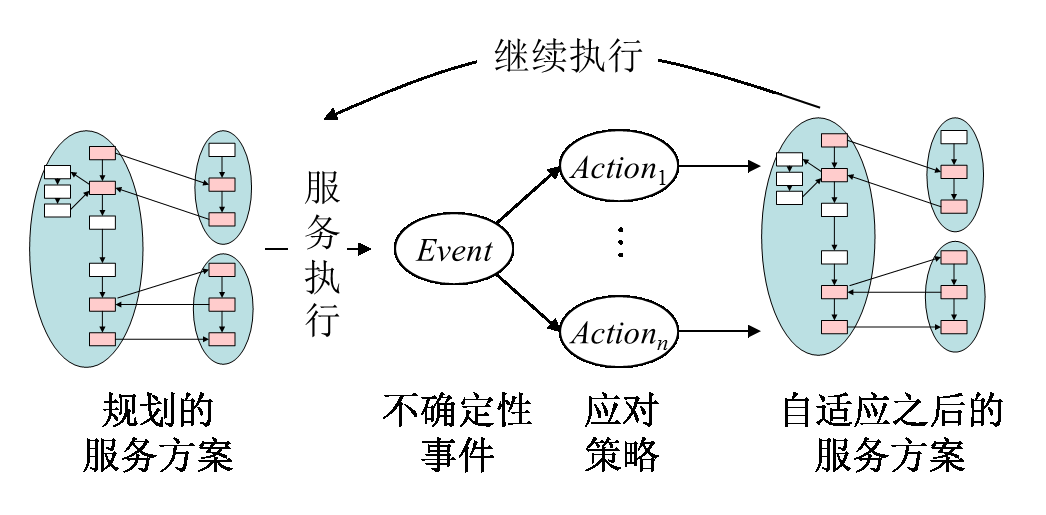
\includegraphics[width = 0.4\textwidth]{uc_plan}
\caption{按需应变的服务不确定性自适应决策}\label{uc_plan}
\vspace{-1em}
\end{figure}

\subsection{课题研究的背景和意义}

在服务执行过程中,对发生的不同类型的不确定性事件可能有多种处理对策(重试、补偿、重组、替换等),不同的对策对服务的影响是不同的。如何以最小的代价使服务尽快回到期望轨道,需要做出最优的选择。另外,由于不确定性是可传播的,选择决策时不能仅考虑到对当前环节的处理,还需要考虑到它对未来的长期影响,从而达到整体最优,因此这是一个长期的动态决策过程。

以民航服务为例。某航班遵循预先制定的时间表进行飞行,若因机械故障导致航班延误(“变”),那么航空公司、售票处、机场、乘客的行为均要随之发生变化,航空公司要根据客户的需求(“需”)指示机场对其进行改签并安排食宿,或要求售票处办理退票、补偿,或者什么也不做(“应”)。这三种对策所造成的后果是不同的,需要根据航班延误的时间、涉及乘客的数目等复杂因素来动态寻求最优决策。

本文根据服务执行中发生的具体不确定性,利用不确定性触发关系图(UTG)刻画不确定性事件所导致的服务状态以及所采取的决策动作之间的转换关系,以服务成功执行的概率最大、时间延迟最小、成本最低作为决策优化的目标,建立基于Markov决策过程(MDP)的不确定性优化决策模型并加以求解,生成对当前服务方案的最优改进策略。
